\section{Navigation Stategy}
This chapter will give a general overview of the software developed for
\textsc{Avalon} and discuss the interaction between control system and path
planner. Sections \ref{sec:sailor} and \ref{sec:navigator} will then go further
into details of the actual controller and path planner respectively.

The core hardware part and the brain of the system on the sailing vessel is the
main computer MPC21 from {\sc DigitalLogic}, a 500\,MHz device with 1024\,MB
RAM and a compact flash hard-drive. The device has an average power consumption
of about 8\,watts, the protection of a metal housing and a total weight of less
than 1\,kg.
% \begin{figure}[htb]
% \centering
% 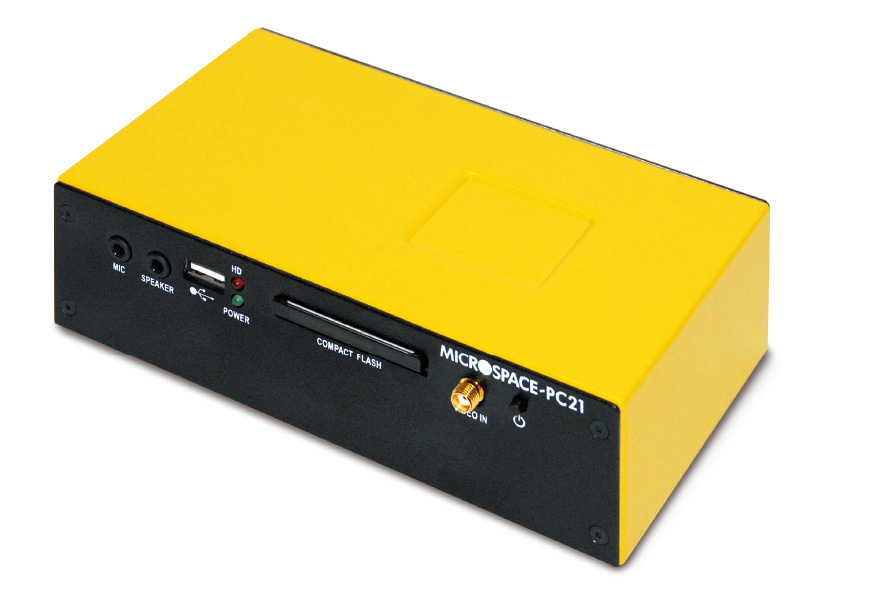
\includegraphics[height=4.0cm]{pics/RE_MPC21.png}\label{fig:mainpc}
% \caption{Main PC and brain of {\sc Avalon}\cite{digitallogic}}
% \end{figure}
%
The base of the entire software structure is the middleware DDX\cite{ddxpaper}
that runs on a Linux Operating System. This software manages a shared memory
called the Store and thus provides a means of communication between individual
programs that all run in parallel (see figure \ref{fig:ddx}). 

Sensor drivers will collect data from the specific sensors (see section
\ref{sec:sensors}) and store it in the DDX Store, from where it can be accessed
by the control and path planning programs.
% 
% A distinct advantage of DDX is the modular software structure. If ever a
% program crashes, it can be restarted without interrupting the other processes.
The different subprograms used on \textsc{Avalon} are depicted in figure
\ref{fig:ddx}.

\begin{figure}[htb]
\centering
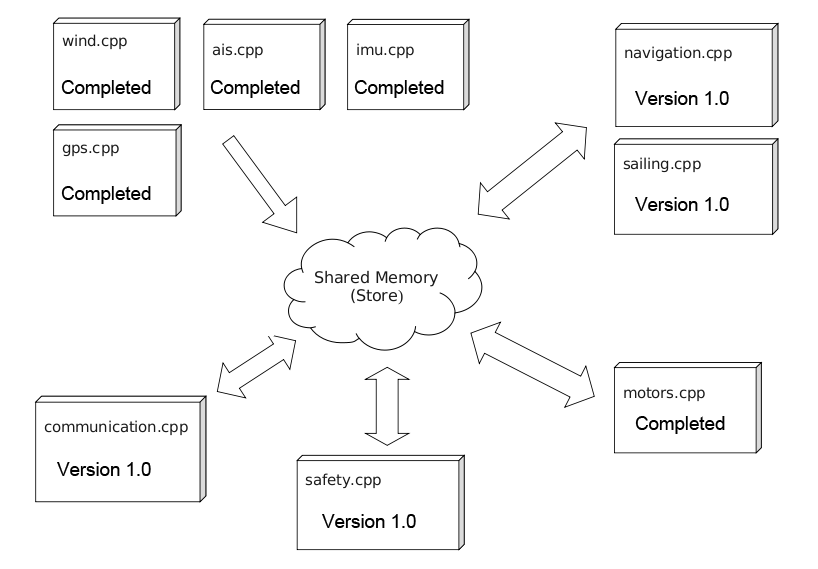
\includegraphics[height=5.5cm]{pics/RE_ddxplain.png}
\caption{Software organisation} \label{fig:ddx}
\end{figure}

%
%
\subsection{Sensors} \label{sec:sensors}
All desired information such as position, heading or speed are measured by
several sensors located all over the boat. To get a fully controllable system,
data is collected from the following sensors:
%
%\begin{description}[\IEEEsetlabelwidth{Wind}\IEEEusemathlabelsep]
%\item[\textbf{GPS}] 
\subsubsection{GPS \& IMU} 
%Provides position, heading and speed. The sensor's antenna is mounted on top of the mast. The electronic unit is located in the hull.
%\item[\textbf{IMU}]
The localization of the boat is performed by an \textit{Inertial Measurement
Unit} (by \textsc{X-Sens}) that is combined with a GPS receiver. Using the
accelerations in all 6 degrees of freedom and a high update rate of 120 Hz,
occasional deviations of the GPS-data will automatically be smoothed out. The
system therefore produces highly accurate positioning.
%
%\item[\textbf{Wind}]
\subsubsection{Wind} Mounted on top of the mast, the wind-sensor provides wind
speed and direction. {\sc Avalon} has an ultrasonic wind-sensor that promises
less mechanical failure than a conventional sensor with a turning wheel. The
sensor by Danish company \textsc{Deif} is IP-66 approved and connected to the
main computer via a RS-485 interface.
%\item[\textbf{AIS}]
\subsubsection{AIS} This Sensor receives data such as position and velocity
from other boats via VHF. The AIS system is an additional means of perception
that ensures that collisions with large commercial ships are avoided.
%\end{description}
%
\subsection{Navigation Management} \label{sec:skipper}
The overall navigation management is being performed by a program further
referred to as trajectory tracker. It's two main tasks are to trigger the local
planner of the path planning algorithm (see section \ref{sec:navigator}) and to
extract from a planned path a sailable boat heading that can be followed by the
controller (see section \ref{sec:sailor}).

The program keeps track of the boat's location as well as it's environment. In
case of predefined emergency cases, it is able to set new destination coordinates.

Having a state machine architecture, the trajectory tracker can switch between
the following states:
%
\subsubsection{Standard Navigation}
If not approaching a target\hide{ or buoy}, this state generates headings for the
control system, going from way-point to way-point. If the wind changes more than $20$°
or if the ship distances itself from the current trajectory for more than a
predefined distance, a new calculation will be initiated. 
\subsubsection{Goal Approach}
If approaching a target position, the trajectory tracker will always send a
heading that is directing exactly towards that point.
\hide{\subsubsection{Buoy Approach}
This is a state designed especially for short course racing. Due to regulations
that always require a port-side surrounding of the regatta buoys, this state
will - when approaching a buoy - always write a heading that will lead the boat
around the buoy.}
\subsubsection{New Calculation}
In this state, the trajectory tracker manages and supervises the new
calculation. After having checked that the new way-points have been stored, it
switches back to \textit{Standard Navigation}
%
%
